\chapter{Sviluppi tecnologici}\label{ch:sviluppi}
Questo capitolo riguarda i miglioramenti realizzati dal punto di vista tecnologico che sono andati direttamente ad impattare la piattaforma AirQino, migliorandone in un caso l'affidabilità dei dati e nell'altro i tempi di risposta del database per query particolarmente onerose.

% Replica del database di produzione
\section{Replica del database di produzione}\label{sec:replica}

Spesso fare analisi mediamente complesse sui dati contenuti in un database può comportare rallentamenti nei tempi di risposta. Se questi carichi risultano frequenti, il sistema può arrivare a bloccarsi e interrompere il servizio.

Una soluzione per risolvere questo problema è la creazione di una (o più) repliche del database primario. Nella replica, i dati e gli oggetti del database vengono copiati e distribuiti su un altro spazio fisico. Le operazioni onerose a questo punto possono essere fatte direttamente sulla replica che agisce come nodo secondario: in questo modo, il carico viene distribuito e non si intaccano le performance del database principale.

Il concetto di \textit{replica} è diverso dal \textit{mirroring}, in cui vengono create una o più copie di un database su diverse istanze del server, e funzionano come copie di riserva (e si attivano soltanto nel caso di guasto del nodo principale).

Un sistema di replica correttamente implementato può offrire diversi vantaggi, tra cui riduzione del carico (perchè i dati replicati possono essere distribuiti su più server), efficienza (i server offrono prestazioni migliori perchè meno gravati da query pesanti) e ridondanza (i dati sono raggiungibili da più indirizzi).

Di contro, questa tecnica comporta la necessità di mantenimento dei nodi secondari, spesso collocati su server diversi (con i costi a questi associati). Inoltre, repliche errate o non implementate in maniera corretta possono causare la mancata sincronizzazione tra i nodi, portando ad una perdita o incoerenza dei dati.

\subsection{Motivazioni}\label{ssec:replica-motivazioni}
La replica offrire vantaggi principalmente legati alle prestazioni, disponibilità e sicurezza dei dati:
\begin{enumerate}
  \item \textbf{Maggiore affidabilità}: tramite la replica del database viene garantita la disponibilità dei dati anche nel caso in cui una delle macchine presenti un guasto hardware. In questo caso, il sistema di gestione del database distribuito deve essere in grado di indirizzare gli utenti interessati ad uno degli altri nodi disponibili;
  \item \textbf{Miglioramento delle prestazioni}: essendo i dati distribuiti su diverse istanze, accessi multipli non saturano i server. Questo aspetto risulta particolarmente importante per applicazioni che possono avere una grande quantità di richieste simultanee;
  \item \textbf{Maggiore sicurezza dei dati}: Mentre in un sistema tradizionale i backup di un database (se effttuati) sono archiviati sullo stesso disco, con la replica del database vengono scritti su più server, aumentandone di fatto l'affidabilità e la ridondanza.
\end{enumerate}

Esistono diverse tecniche di replicazione del database, che dipendono sia dalla tecnologia utilizzata (MySQL, Postgres) che dalla natura del database stesso (relazionale o non relazionale). Il database di AirQino fa uso di Timescale\footnote{Timescale: Time-series data simplified - \url{https://www.timescale.com}}, basato su Postgres; una caratteristica di Postgres è la possibilità di replicazione con la tecnologia di \textbf{Streaming Replication}, descritta di seguito.

\subsection{Streaming Replication}\label{ssec:streaming-replication}
La streaming replication di PostgreSQL è una funzionalità che consente di replicare i dati in tempo reale da una istanza di PostgreSQL a un'altra. Questo significa che, se si modificano i dati in una delle istanze, questi saranno immediatamente replicati anche nell'altra istanza. Questa istanza database di replica di lettura ("standby" in termini PostgreSQL) è una replica fisica creata in modo asincrono dell'istanza del database primario.

PostgreSQL fa utilizza un ruolo di "replica" (\textit{replication role}) per eseguire la replica in streaming (il ruolo presenta dei privilegi ma non può essere utilizzato per modificare i dati, la replica infatti è di sola lettura).

La replica si basa sulle transazioni WAL (Write Ahead Log) e utilizza il protocollo TCP per garantire una connessione sicura tra i server e inviare in modo asincrono le modifiche al database via via che vengono effettuate.

È possibile promuovere una replica di lettura PostgreSQL a una nuova istanza database di origine. Una volta promossa, la replica smette di ricevere comunicazioni WAL e non è più un'istanza di sola lettura.

PostgreSQL salva le informazioni aggiornate del server primario in registro delle transazioni, noto come registro \textit{write-ahead}, utile in preparazione per il ripristino da crash o il rollback. La replica in streaming funziona proprio trasferendo e applicando il WAL al server di replica in tempo reale.

\begin{figure}[H]
\centering
\captionsetup{justification=centering}
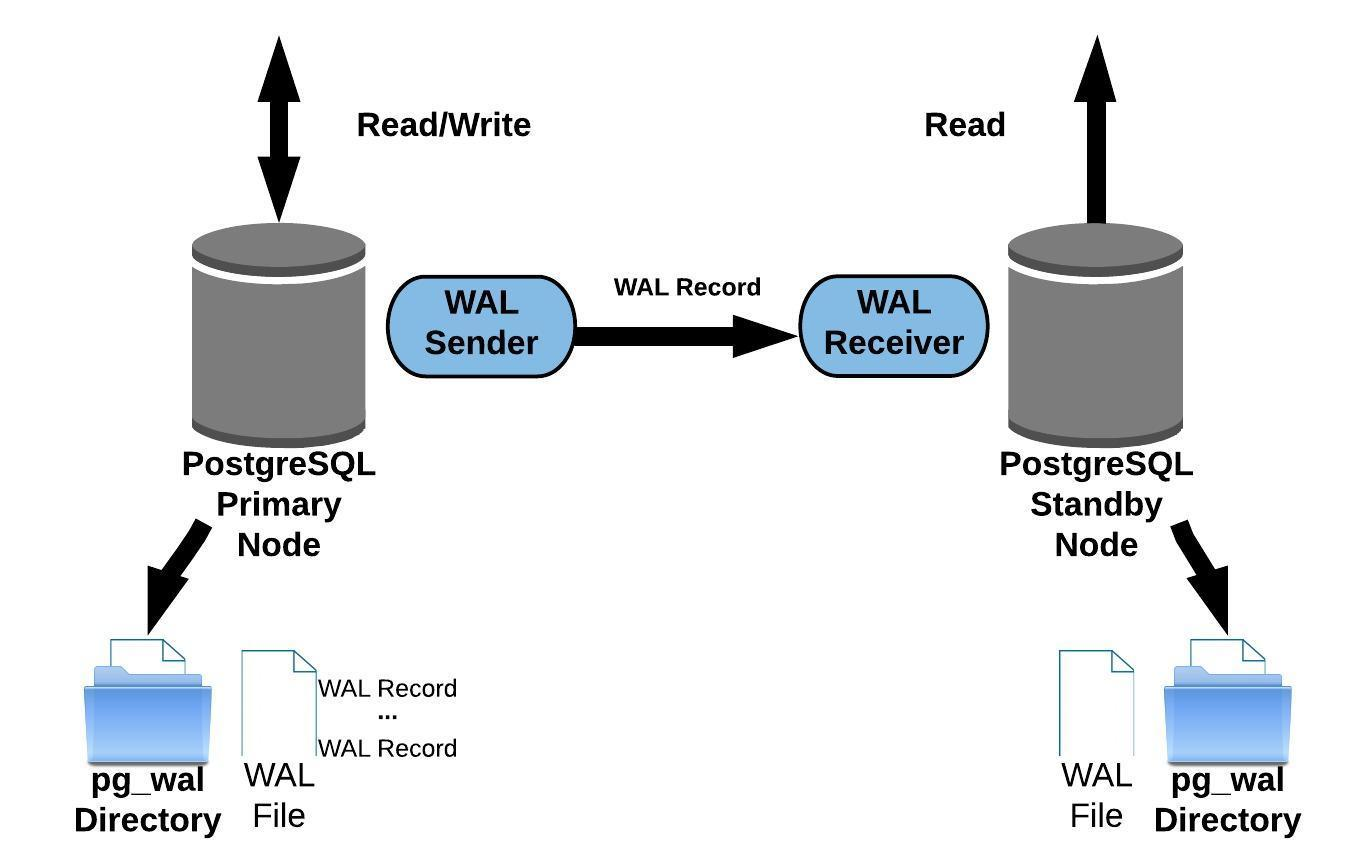
\includegraphics[width=0.75\textwidth,height=\textheight,keepaspectratio]{img/streaming_replication.jpg}
\caption{Streaming Replication di PostgreSQL\\Fonte: \url{https://severalnines.com}}
\label{fig:streaming-replication}
\end{figure}

La replica in streaming può essere costruita in una configurazione 1:N, in cui è configurabile un solo server primario, ma è possibile configurare più server di replica (configurazione \textit{multi-standby}). È anche possibile creare una configurazione a cascata in cui un server di replica si connette ad un altro server di replica.

Per la replica in streaming, è possibile scegliere se effettare una replica sincrona o asincrona. La differenza tra replica sincrona e replica asincrona sta nell'attesa o meno della risposta dal server di replica prima di completare l'elaborazione sul server primario:
\begin{itemize}
  \item \textbf{Replica sincrona}: il server primario attende una risposta dal server di replica prima di completare un processo. In questo caso il tempo di risposta complessivo include anche il tempo di spedizione del registro;
  \item \textbf{Replica asincrona} (impostazione predefinita): il server primario completa un processo senza attendere una risposta dal server di standby. Pertanto, il tempo di risposta complessivo è più o meno lo stesso di quando non viene utilizzata la replica in streaming; in questa modalità il risultato aggiornato sul server primario potrebbe non essere immediatamente disponibile sul server di replica. \cite{streaming_replication}
\end{itemize}

Esistono di contro diverse limitazioni per le repliche con PostgreSQL:
\begin{itemize}
  \item Ogni replica di lettura PostgreSQL è di sola lettura. Non è possibile creare una replica di lettura che sia scrivibile;
  \item Non è possibile creare una replica di lettura da un'altra replica di lettura a cascata;
  \item Gli utenti e i ruoli di accesso vengono rispecchiati dall'istanza primaria, il che significa che non è possibile utilizzare credenziali diverse o aggiungere utenti aggiuntivi soltanto alla replica;
  \item Non è possibile creare tabelle e viste nell'istanza di replica; in pratica dalla replica si possono solo eseguire query di tipo \textit{SELECT}.
\end{itemize}

\subsubsection{Preparazione del database primario}

\begin{enumerate}
  \item Per avviare la procedura si crea sul database un utente PostgreSQL con un ruolo adatto ad avviare la streaming replication:
  \vspace{1mm}
   \begin{lstlisting}[language=sql]
SET password_encryption = 'scram-sha-256'; 
CREATE ROLE repuser WITH REPLICATION PASSWORD 'SOME_SECURE_PASSWORD' LOGIN;\end{lstlisting}
  \item Aggiungere i seguenti parametri al file \url{/var/lib/postgresql/data/postgresql.conf}:
  \vspace{1mm}
  \begin{lstlisting}[]
listen_addresses= '*'
wal_level = replica
max_wal_senders = 2
max_replication_slots = 2
synchronous_commit = off
\end{lstlisting}

  \item Aggiungere i seguenti parametri al file di configurazione \url{/var/lib/postgresql/data/pg_hba.conf} per configurare l'autenticazione basata su host in modo da accettare connessioni dalla replica\footnote{Dalla documentazione Streaming Replication: \url{https://www.postgresql.org/docs/current/warm-standby.html\#STREAMING-REPLICATION}}:
  \vspace{1mm}
\begin{lstlisting}[]
host     replication     repuser   <REPLICA_IP>/32       scram-sha-256
\end{lstlisting}
dove \textit{repuser} è l'utente creato al passo 1 e \textit{REPLICA\_IP} è l'IP della macchina in cui si trova la replica;
  \item Riavviare il database per applicare i cambiamenti;
  \item Infine creare uno slot di replicazione sul database:
  \vspace{1mm}
  \begin{lstlisting}[language=sql]
SELECT * FROM pg_create_physical_replication_slot('replica_1_slot');
\end{lstlisting}
\end{enumerate}

\subsubsection{Configurazione della replica}

\begin{enumerate}
  \item Stoppare l'istanza Postgres:
  \vspace{1mm}
\begin{lstlisting}[]
pg_ctl -D $PGDATA -m fast -w stop
\end{lstlisting}
  \item Cancellare i contenuti della cartella PGDATA:
  \vspace{1mm}
\begin{lstlisting}[]
rm -rf $PGDATA/*
\end{lstlisting}
  \item Avviare il backup del database primario:
  \vspace{1mm}
\begin{lstlisting}[]
pg_basebackup -h <PRIMARY_HOST> -p <PRIMARY_PORT> -D $PGDATA -U repuser -vP -R -W
\end{lstlisting}
Dove \textit{PRIMARY\_HOST} è l'IP della macchina in cui si trova il database primario, \textit{PRIMARY\_PORT} è la porta del database primario e \textit{repuser} è l'utente di replicazione creato al passo 1.
Verrà chiesta in maniera interattiva la password di replicazione impostata sempre al passo 1 di preparazione (\textit{SOME\_SECURE\_PASSWORD});
  \item Infine avviare l'istanza Postgres:
  \vspace{1mm}
\begin{lstlisting}[]
pg_ctl -D $PGDATA -w start
\end{lstlisting}
A questo punto la replica dovrebbe essere funzionante e sincronizzata 1:1 in tempo reale con il db primario.
\end{enumerate}

\subsubsection{Automazione con Docker}
L'intero setup (sia database primario che la replica) può essere automatizzato con Docker e docker-compose.
Poichè i passi per creare la replica richiedono di stoppare l'istanza Postgres, non si può eseguire all'interno del container Docker già avviato perchè si stopperebbe tutto il container.
Per questo è necessario dare i comandi per la replica da uno script di \textit{entrypoint} che viene eseguito prima di avviare il container.
\begin{enumerate}
  \item Creare un Dockerfile da immagine base Timescale con l'aggiunta di uno script entrypoint così strutturato:
  \vspace{1mm}
  \begin{lstlisting}[]
FROM timescale/timescaledb:latest-pg13
ADD replica.sh /docker-entrypoint-initdb.d/
\end{lstlisting}
  \item Creare il file \url{replica.sh} che viene eseguito tutte le volte che si avvia il database:
  \vspace{1mm}
  \begin{lstlisting}[]
echo "Stopping Postgres instance..." 
pg_ctl -D ${PGDATA} -m fast -w stop

echo "Clearing PGDATA folder..." 
rm -rf ${PGDATA}

echo "Creating base backup..." 
PGPASSWORD=${REPLICATION_PASSWORD} pg_basebackup -h ${REPLICATION_HOST} -p ${REPLICATION_PORT} -D ${PGDATA} -U ${REPLICATION_USER} -vP -R -w

echo "Restarting Postgres instance..." 
pg_ctl -D ${PGDATA} -w start
\end{lstlisting}
La flag -W di pg\_basebackup chiede la password in maniera interattiva, che non funziona per script automatizzati. Come alternativa si può usare la flag -w (minuscola) e passare la password come variabile di ambiente \textit{PGPASSWORD};
\item Creare il file docker-compose.yml:
\vspace{1mm}
  \begin{lstlisting}[]
services:
  replica:
    build:
        context: .
        dockerfile: Dockerfile
    environment:
        # Cartella PDATA custom
        PGDATA: /var/lib/postgresql/data/pgdata

        # Parametri di replicazione
        REPLICA_USER: repuser # Utente di replicazione impostato al punto 1
        REPLICATION_HOST: x.x.x.x # IP del db primario
        REPLICATION_PORT: x # Porta del db primario
        REPLICATION_PASSWORD: SOME_SECURE_PASSWORD # Password di replicazione impostata al punto 1
    ports:
        - 45432:5432
    volumes:
        - /var/replica-pg13-timescale/:/var/lib/postgresql/data
\end{lstlisting}

  \item Avviare il container con \url{docker-compose} \url{up}.
\end{enumerate}

Allo stesso modo è possibile automatizzare con Docker anche il database primario.

% Ottimizzazione di query temporali
\section{Ottimizzazione di query temporali}\label{sec:cont-aggr}
\ldots

\subsection{Motivazioni}\label{ssec:cont-aggr-motivazioni}
\ldots

\subsection{Continuous Aggregates}\label{ssec:cont-aggr}
I continuous aggregate sono una funzionalità integrata in TimescaleDB che consente di aggregare i dati in tempo reale, senza la necessità di eseguire query aggiuntive. Questa funzionalità utilizza i contatori per tenere traccia dei dati aggregati in tempo reale e fornisce una rappresentazione dei dati aggregati in tempo reale.

I continuous aggregate offrono numerosi vantaggi, tra cui:

- Flessibilità: è possibile aggregare dati in tempo reale in base a qualsiasi criterio desiderato.

- Risparmio di tempo: non è necessario eseguire query aggiuntive per ottenere informazioni aggregate in tempo reale.

- Risparmio di spazio: i dati aggregati in tempo reale occupano meno spazio rispetto ai dati non aggregati.

- Maggiore efficienza: i continuous aggregate sono più efficienti dei query batch per l'aggregazione dei dati in tempo reale.

\subsection{Risultati ottenuti}\label{ssec:cont-aggr-risultati}
\ldots